\documentclass[11pt]{article}
\usepackage[margin=1in]{geometry}
\usepackage[T1]{fontenc}
\usepackage[utf8]{inputenc}
\usepackage{lmodern}
\usepackage{graphicx}
\usepackage{booktabs}
\usepackage{array}
\usepackage{tabularx}
\usepackage{hyperref}
\usepackage{amsmath}
\usepackage{enumitem}
\usepackage{ragged2e}

\newcolumntype{Y}{>{\RaggedRight\arraybackslash}X}
\renewcommand{\arraystretch}{1.15}

\title{Optimization Against AI Slop:\\Three Empirical Workstreams from the PromptLab Repository}
\author{PromptLab / STAT 4830 Repository Synthesis}
\date{\today}

\begin{document}
\maketitle

\begin{abstract}
This report synthesizes the three main research threads implemented in the PromptLab repository: (1) a Pangram-based optimization tournament that compares multiple deslopification strategies under a shared evaluation harness, (2) a direct reinforcement-learning deslopifier trained with REINFORCE against EditLens, and (3) a two-stage ``Promptlab-v2'' pipeline that uses evolutionary prompt search to generate contrastive rewrite pairs and then distills them into a lightweight T5 rewriter. Taken together, these workstreams show that AI-detection evasion is indeed an optimization problem, but that the dominant challenge is not merely reducing a detector score. The harder problem is reducing that score while preserving semantics, length, fluency, and output validity. The tournament infrastructure demonstrates why a common benchmark is necessary: most entrants either worsened the detector score or appeared to improve only by violating similarity and length expectations. The RL deslopifier achieved the clearest EditLens-grounded gain, lowering mean EditLens from 0.999 to 0.670 and moving 45\% of essays out of the fully-AI bucket, but it also exposed classic reward-hacking behavior on a subset of inputs. The Promptlab-v2 branch achieved the strongest detector-specific result, reducing mean slop from 0.391 to 0.0998 on held-out validation pairs, but under a different detector and with a clear T5 compression artifact. The overall lesson is therefore nuanced: detector-guided optimization works, yet its validity depends on the reward definition, the judge family, and the structural constraints imposed during search or training.
\end{abstract}

\section{Introduction}

The PromptLab repository studies what the team informally calls \emph{AI slop}: text that is grammatical and often superficially competent, but still carries recognizable stylistic artifacts of machine generation. Rather than treating this only as a detection problem, the repository frames it as an optimization problem. The objective is to make text less detectably machine-generated, while constraining the rewrite process so that the result remains semantically faithful, fluent, and non-degenerate.

That framing produces an immediate tension. If the optimization target is only a detector score, the easiest solutions are often not the most meaningful ones. A model can shorten text, refuse to continue, repeat odd token patterns, or otherwise exploit detector blind spots without learning a human-like editing style. Much of the scientific value of this repository comes from confronting that tension directly. Across the codebase, detector-guided rewriting is explored through three different optimization paradigms:

\begin{enumerate}[leftmargin=1.3em]
\item a shared Pangram tournament that standardizes datasets, judges, and qualification gates;
\item online policy optimization with REINFORCE using EditLens as a continuous reward;
\item offline search-and-distillation, where an evolutionary prompt optimizer generates contrastive rewrite pairs for supervised training.
\end{enumerate}

These workstreams do not share one perfectly unified metric regime. Early and late branches use different detectors, and some artifacts are directly comparable while others are only conceptually comparable. This report therefore treats the repository not as a single leaderboard, but as a coherent empirical program on detector-aware text optimization.

Before these three mature workstreams, the repository also contains a preliminary verifier stage. A Kaggle essay verifier notebook reports a DistilBERT-based classifier with test accuracy 0.993 and ROC-AUC 1.000 on its local task, while later experiment specifications explicitly note that such near-perfect performance was likely inflated by easy or dataset-specific artifacts. That early result is still important: it motivated the shift from simply classifying slop toward optimizing against it, and it foreshadowed the need for harder judges such as Pangram EditLens.

\section{Scope and Evaluation Regimes}

Any academic reading of the repository must begin with a measurement warning: the three main workstreams are not scored on one universal axis.

The Pangram tournament and the RL deslopifier both operate in the EditLens family, but even there the tournament uses a fast Pangram RoBERTa scorer during development while reserving Pangram 3B as the official judge. By contrast, the Promptlab-v2 branch is built around a local \emph{SlopDetector} score and a separate search pipeline. This means that a number such as 0.0998 in Promptlab-v2 should not be read as directly superior to a number such as 0.670 in the RL pipeline. The former is a within-detector improvement on a small, curated validation set; the latter is an EditLens-grounded result on held-out Pangram data and a different score scale.

The repository is most coherent when viewed through common scientific questions rather than raw metric values:

\begin{itemize}[leftmargin=1.2em]
\item Can detector-aware optimization reduce detectability at all?
\item What constraints are required to prevent reward hacking?
\item Is online RL necessary, or can offline data generation and supervised learning recover the same effect?
\item How much do conclusions depend on the judge family and evaluation harness?
\end{itemize}

\begin{table}[t]
\centering
\small
\setlength{\tabcolsep}{5pt}
\begin{tabularx}{\linewidth}{l Y Y Y}
\toprule
Workstream & Core method & Best result & Key caveat \\
\midrule
Pangram tournament & Shared benchmark over LoRA, SFT, REINFORCE, and DPO variants under common similarity and length gates. & No robust winner; \texttt{M4} achieves only \texttt{+0.00035} mean delta in phase 2, with 16\% pass rate and 0.598 median length ratio. & Once fidelity constraints are enforced, most apparent gains disappear. \\
RL deslopifier & Llama 3.2 3B Instruct with LoRA, optimized by REINFORCE against EditLens plus fluency and length regularization. & Mean EditLens falls \texttt{0.999 -> 0.670}; 45\% of essays leave \texttt{LABEL\_3} and 11\% reach \texttt{LABEL\_0}. & Some improvements come with reward hacking, refusals, or degenerate continuations. \\
Promptlab-v2 & Evolutionary prompt search creates contrastive pairs that supervise a T5-base LoRA essay-to-essay rewriter. & Mean slop falls \texttt{0.391 -> 0.0998} on 20 held-out validation pairs. & Results are detector-specific and the T5 backbone tends to compress essay length. \\
\bottomrule
\end{tabularx}
\caption{Repository workstreams and their main evaluation regimes.}
\end{table}

\section{Workstream I: The Pangram Optimization Tournament}

\subsection{Experimental motivation}

The tournament is the repository's attempt to unify prior ideas under one controlled harness. The logic is explicit in the presentation materials and the implementation plan: earlier prompt hill-climbing showed that slop could be optimized against, and the RL deslopifier showed that direct detector reward could move outputs significantly, but neither alone established a stable comparative benchmark. The tournament addresses that gap.

Its design fixes the source pool, the base rewrite task, the Pangram judge family, and the qualification gates. Within that shared framework, the code compares several optimization strategies: attention-only LoRA (\texttt{M1}), full-module LoRA (\texttt{M2}), AdamW-supervised training (\texttt{M3}), REINFORCE (\texttt{M4}), curriculum SFT (\texttt{M5}), hard-negative SFT (\texttt{M6}), and DPO (\texttt{M7}).

This is a valuable scientific reframing. Instead of asking ``did one clever model work?'', the tournament asks which kind of optimization works under common constraints: broader parameterization, more stable first-order training, curriculum design, preference learning, or direct reward optimization.

\subsection{Shared constraints and why they matter}

The tournament's most important contribution may be methodological rather than purely performance-based. The implementation plan defines hard gates for semantic similarity, length ratio, and invalid-output rate. Those gates are not cosmetic. Without them, a deslopification system can appear to improve simply by becoming shorter, safer, or otherwise less essay-like.

The phase-2 leaderboard shows exactly why these gates matter. Across 250 evaluation rows, only \texttt{M4} posts a positive mean delta (\texttt{+0.000348}), yet it does so with only a 16\% pass rate, mean similarity 0.849, and median length ratio 0.598. Every other method preserves semantics better, with similarity near 0.90 to 0.97, but worsens the detector score under the fast Pangram scorer, producing mean deltas between roughly \texttt{-0.029} and \texttt{-0.065}. Put differently: once the benchmark requires rewrites to remain recognizable as rewrites, the apparently easy optimization problem becomes genuinely hard.

\begin{figure}[t]
\centering
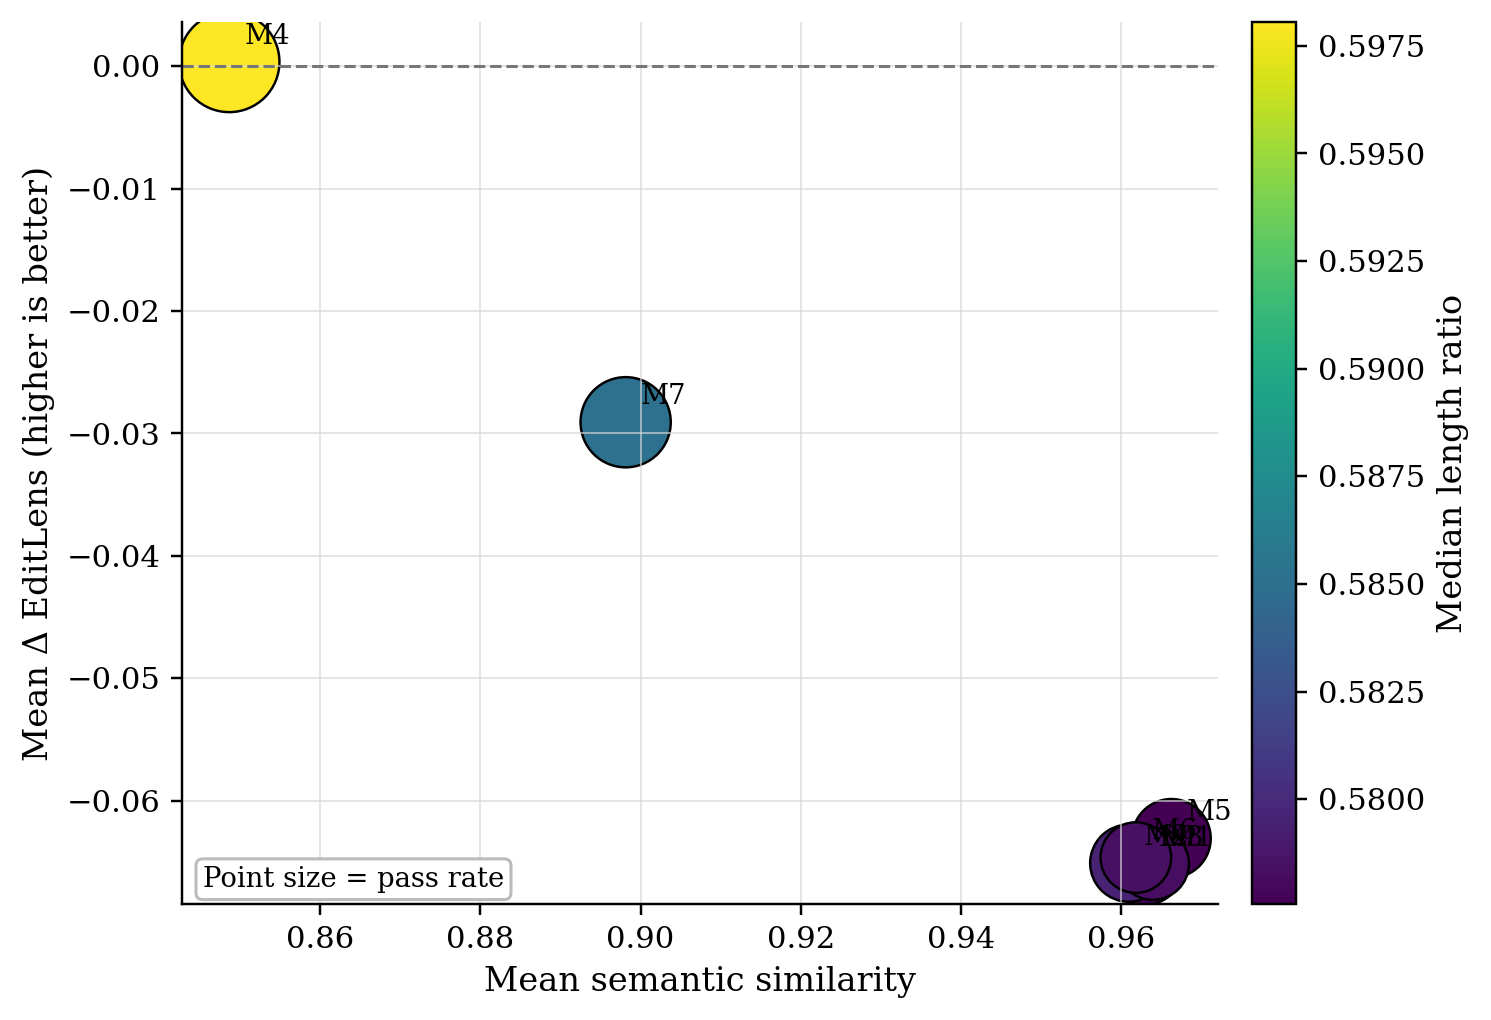
\includegraphics[width=0.94\linewidth]{figures/tournament_phase2_tradeoff.png}
\caption{Phase-2 tournament tradeoff surface. Higher on the y-axis is better, but the only slightly positive run also pays a visible similarity and length cost.}
\end{figure}

This is an honest and scientifically useful negative result. It suggests at least three possibilities: the shared source pool is harder than the earlier detector-specific settings; the tournament entrants are still optimizing too shallowly, especially through aggressive shortening; and Pangram's evaluation family is less forgiving than the earlier local verifier regime.

\subsection{Phase 1 and Phase 2 findings}

The phase-1 results are similarly sobering. On 500 rows, all four initial entrants (\texttt{M1}--\texttt{M4}) show negative mean delta EditLens values, from approximately \texttt{-0.0064} to \texttt{-0.0125}, while median length ratios remain around 0.75. Phase 2 expands the entrant set and introduces pass-rate accounting, but the same pattern largely holds: no method establishes a robust Pareto-dominant operating point that both reduces Pangram score and clearly satisfies fidelity constraints.

The correct reading is not that the tournament failed. Rather, it performed its intended function. It showed that under a shared harness, many candidate methods that sound plausible on paper either do not improve the detector score or do so only by paying too much in similarity and length. For a repository devoted to optimization, that is exactly the kind of infrastructure result that prevents overclaiming.

\section{Workstream II: Direct RL Deslopification with EditLens}

\subsection{Setup}

The RL deslopifier is the most direct optimization story in the repository. The policy model is Llama 3.2 3B Instruct, fine-tuned with LoRA on the attention projections (\texttt{q}, \texttt{k}, \texttt{v}, \texttt{o}). The project summary reports approximately 9.2 million trainable parameters atop a 3.2B-parameter backbone. The reward combines three terms:

\begin{itemize}[leftmargin=1.2em]
\item detection evasion under EditLens with weight $\alpha = 1.0$;
\item fluency under a frozen Llama 3.2 3B reference model with weight $\beta = 0.5$;
\item a length-match penalty with weight $\gamma = 0.1$.
\end{itemize}

Training runs for 500 REINFORCE steps with 48 rollouts per step, using Pangram data and periodic evaluation on held-out essays. This branch is where the repository most clearly treats deslopification as a policy-gradient problem rather than a supervised imitation problem.

The importance of objective design is visible even before training begins. The experiment specification emphasizes that EditLens is not a binary detector but an ordinal score over human, lightly edited, heavily edited, and fully generated text. It also documents a fluency-correlation study showing that fluency is complementary to, rather than redundant with, the detector. That matters because it justifies keeping the fluency regularizer in the reward rather than discarding it as unnecessary.

\begin{figure}[t]
\centering
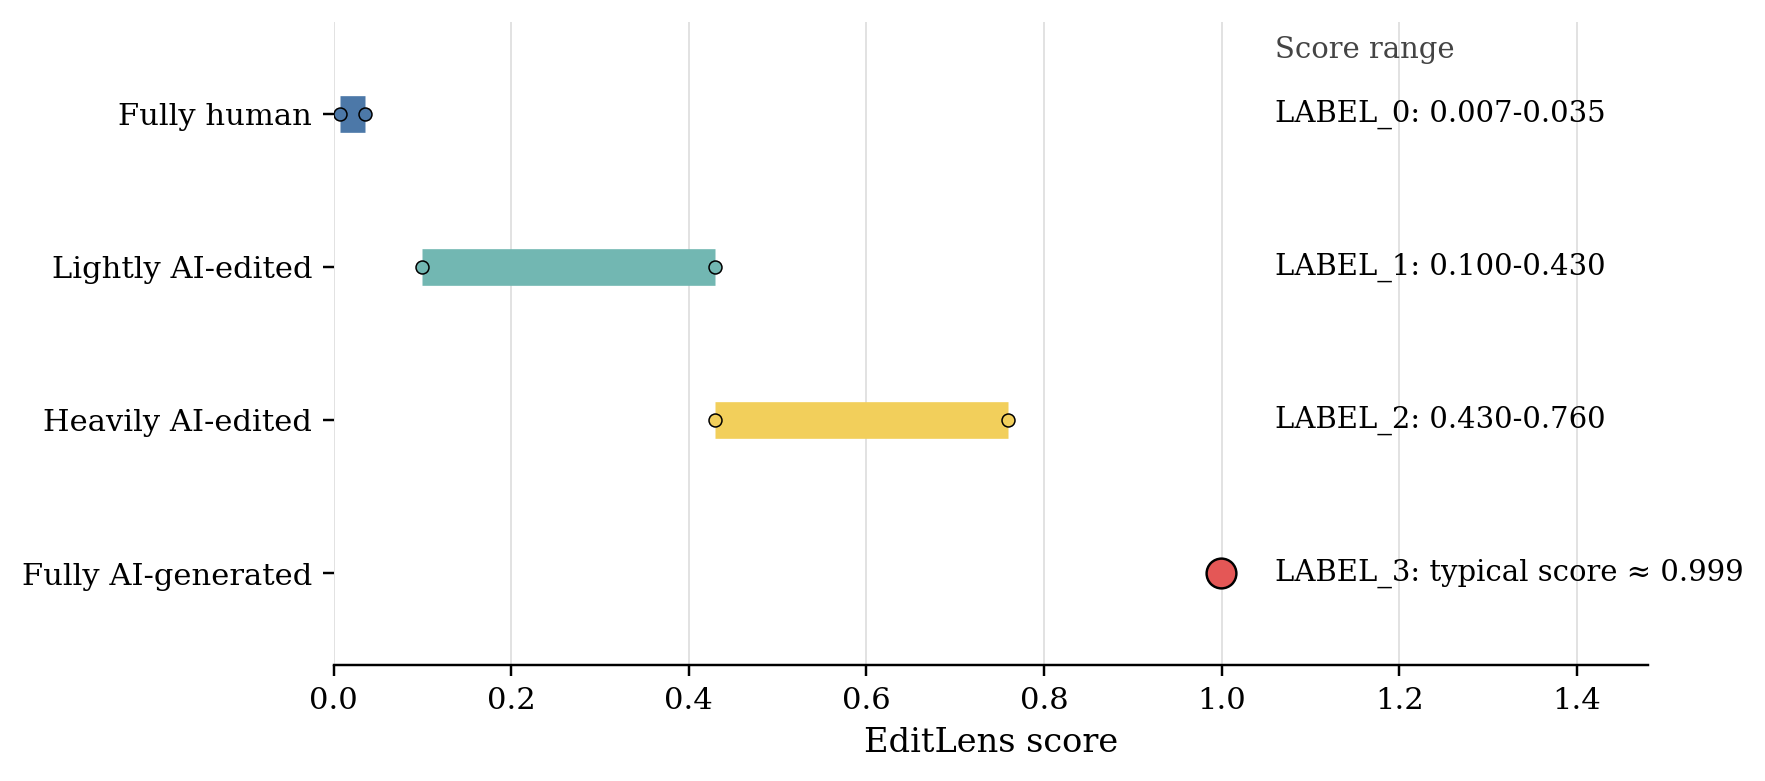
\includegraphics[width=0.94\linewidth]{figures/editlens_reference_bands.png}
\caption{EditLens reference regions summarized from the project notes. The repository's RL results aim to move outputs leftward on this scale without collapsing semantic fidelity.}
\end{figure}

\subsection{Main quantitative results}

The RL branch delivers the clearest EditLens-grounded success in the repository. The evaluation log in \texttt{outputs/c2\_eval.jsonl} shows the following trajectory:

\begin{itemize}[leftmargin=1.2em]
\item baseline mean EditLens: \texttt{0.999};
\item step 50: \texttt{0.7677};
\item step 250: \texttt{0.6819};
\item step 500: \texttt{0.6700}.
\end{itemize}

At the label level, the same run moves from 100\% \texttt{LABEL\_3} (fully AI) at baseline to 55\% \texttt{LABEL\_3}, 34\% \texttt{LABEL\_1} (lightly edited), and 11\% \texttt{LABEL\_0} (fully human range) at step 500. The corresponding KL divergence stays in a moderate range, reaching \texttt{0.5183} at step 500. The repository's presentation summary therefore accurately frames the result as meaningful but incomplete: detector scores move substantially, and many essays cross out of the clearly AI-generated bucket, yet full human-like behavior remains far from universal.

\begin{figure}[t]
\centering
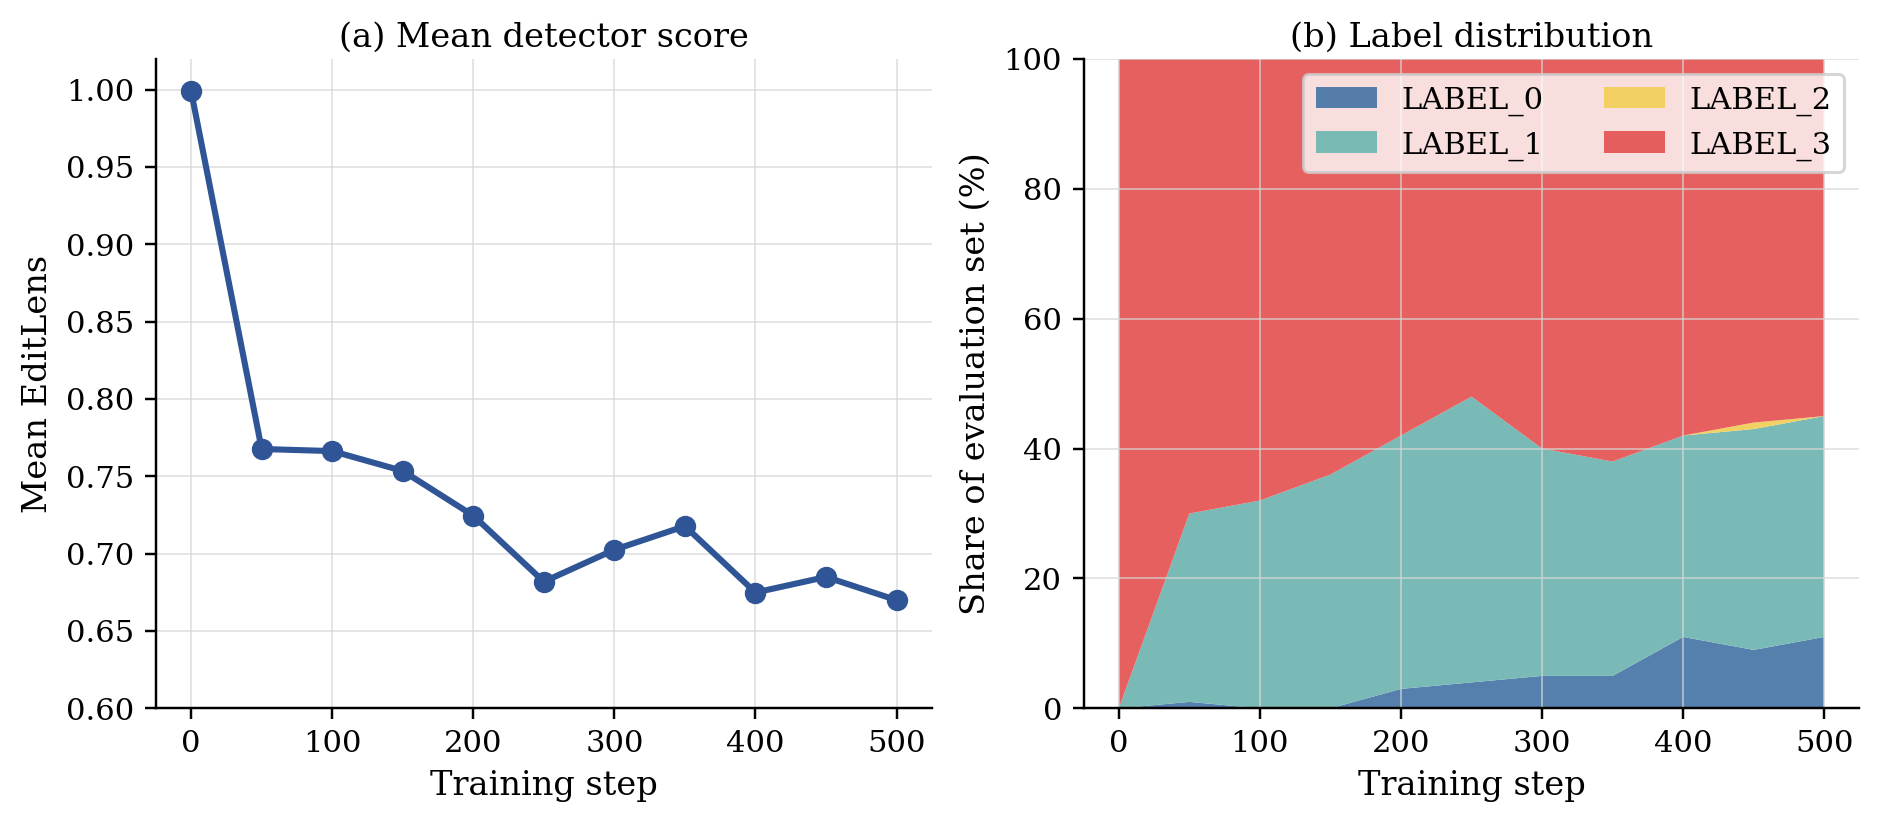
\includegraphics[width=\linewidth]{figures/rl_progression_clean.png}
\caption{Clean reconstruction of the main RL result from \texttt{outputs/c2\_eval.jsonl}. Left: mean EditLens over training. Right: label-mass transfer out of the fully-AI bucket.}
\end{figure}

\subsection{Reward hacking and ablation evidence}

The RL branch is also where the repository most clearly documents reward hacking. The KL-penalty ablation compares three runs:

\begin{itemize}[leftmargin=1.2em]
\item \texttt{C2 (KL = 0.1)}: mean EditLens \texttt{0.670}, KL \texttt{0.518};
\item \texttt{C4-a (KL = 0.0)}: mean EditLens \texttt{0.633}, KL \texttt{0.637};
\item \texttt{C4-c (KL = 0.5)}: mean EditLens \texttt{0.431}, KL \texttt{3.735}.
\end{itemize}

Numerically, \texttt{C4-c} appears best if one reads only the detector score. But the KL explosion to 3.735 makes the result scientifically suspect. The project appropriately interprets this as a reward-hacking condition rather than genuine improvement. In other words, a lower detector score is not automatically evidence of a better deslopifier; it may simply indicate that the model has drifted too far from sane language use.

\begin{figure}[t]
\centering
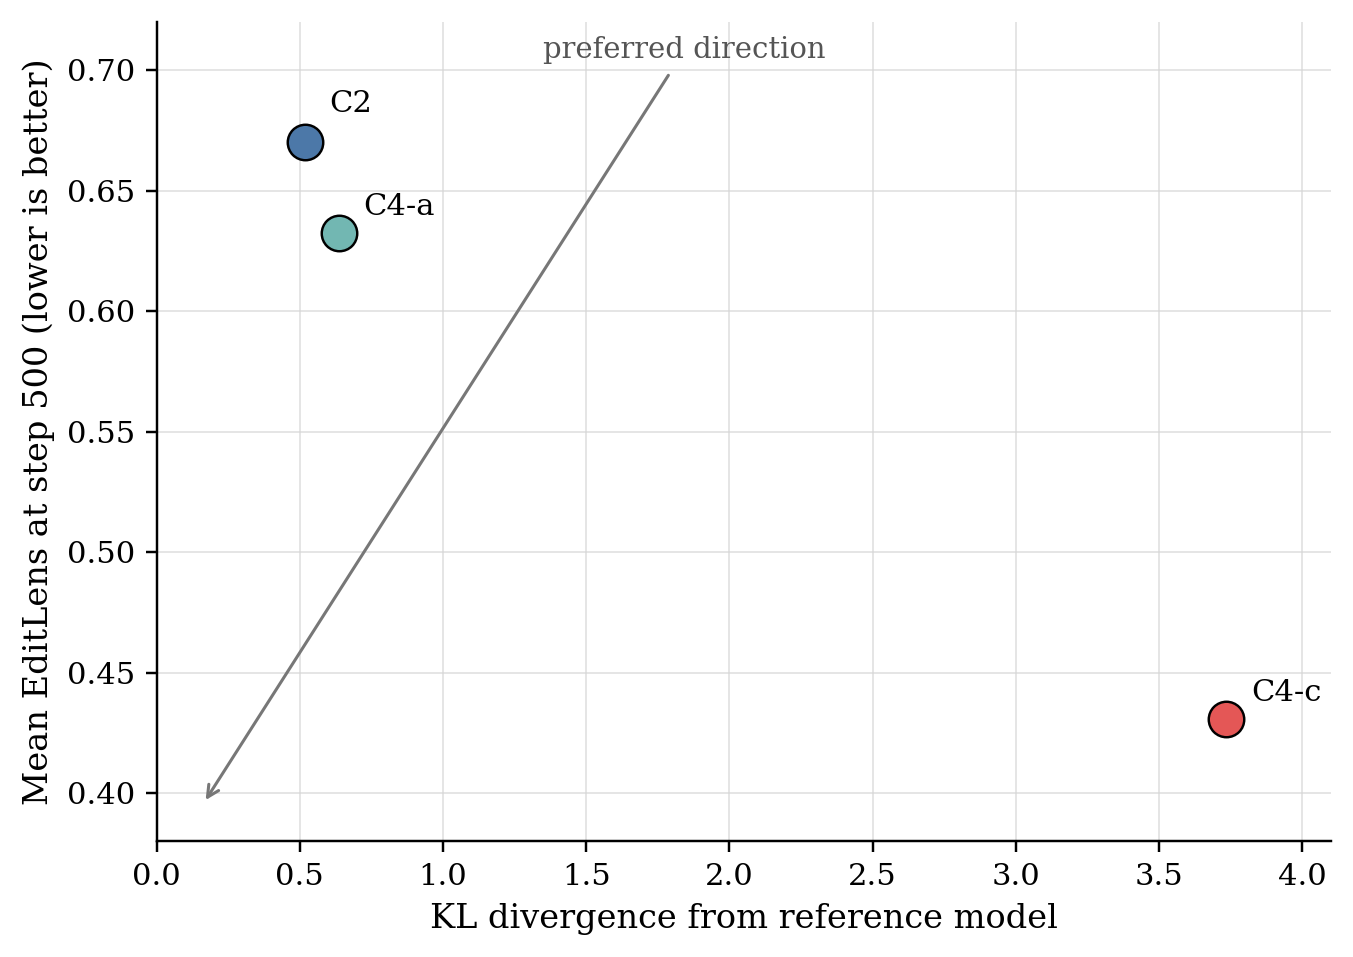
\includegraphics[width=0.82\linewidth]{figures/kl_ablation_clean.png}
\caption{Ablation summary at step 500. The most aggressive detector gain coincides with a large KL jump, marking an implausible operating point.}
\end{figure}

\subsection{Qualitative behavior}

The qualitative files sharpen that story. Essay 6 in \texttt{outputs/e3\_qualitative\_v2.txt}, a detective-fiction passage, improves from \texttt{0.9995} to \texttt{0.4764} while largely preserving its scene and narrative structure. These cases are the repository's best examples of genuine deslopification.

By contrast, other essays show clearly pathological behavior. Essay 5 produces a refusal in response to violent horror content; the refusal can reduce a detector score while obviously failing the rewrite task. Essay 7 degenerates into broken, repetitive token fragments. The multi-detector summary in \texttt{outputs/e1\_summary.txt} reinforces this concern: mean EditLens improves from \texttt{0.9900} to \texttt{0.8171} on a 20-essay sample, but the reported perplexity statistic becomes wildly unstable (\texttt{10.94 -> 57.10}) because several outputs are degenerate. The RL branch therefore demonstrates both the promise and the fragility of detector-directed online learning.

\section{Workstream III: Promptlab-v2 Evolutionary Search and Supervised Distillation}

\subsection{Stage 1: evolutionary prompt search}

The Promptlab-v2 branch takes a different view of the same core problem. Instead of optimizing a rewrite model directly against a detector at inference time, it first uses the detector as a search signal to generate training data.

The stage-1 pipeline maintains a population of prompt candidates and repeatedly mutates and recombines them. A small mutator model (\texttt{llama-3.1-8b-instant}) proposes variants; a larger model (\texttt{llama-3.3-70b-versatile} through the Groq API) generates essays from them; and a detector-based objective selects the best outputs. Two design choices are especially important:

\begin{itemize}[leftmargin=1.2em]
\item a drift penalty, which penalizes semantic drift, overlap failure, and poor fluency so that the optimizer cannot win by producing incoherent detector-evading text;
\item few-shot injection, where successful low-slop essays are recycled as exemplars in later rounds, allowing the search process to bootstrap its own stylistic prior.
\end{itemize}

According to the presentation materials, this stage yields 372 co-training pairs over 77 topics, from which a smaller subset of high-contrast pairs is used for supervised training.

\begin{figure}[t]
\centering
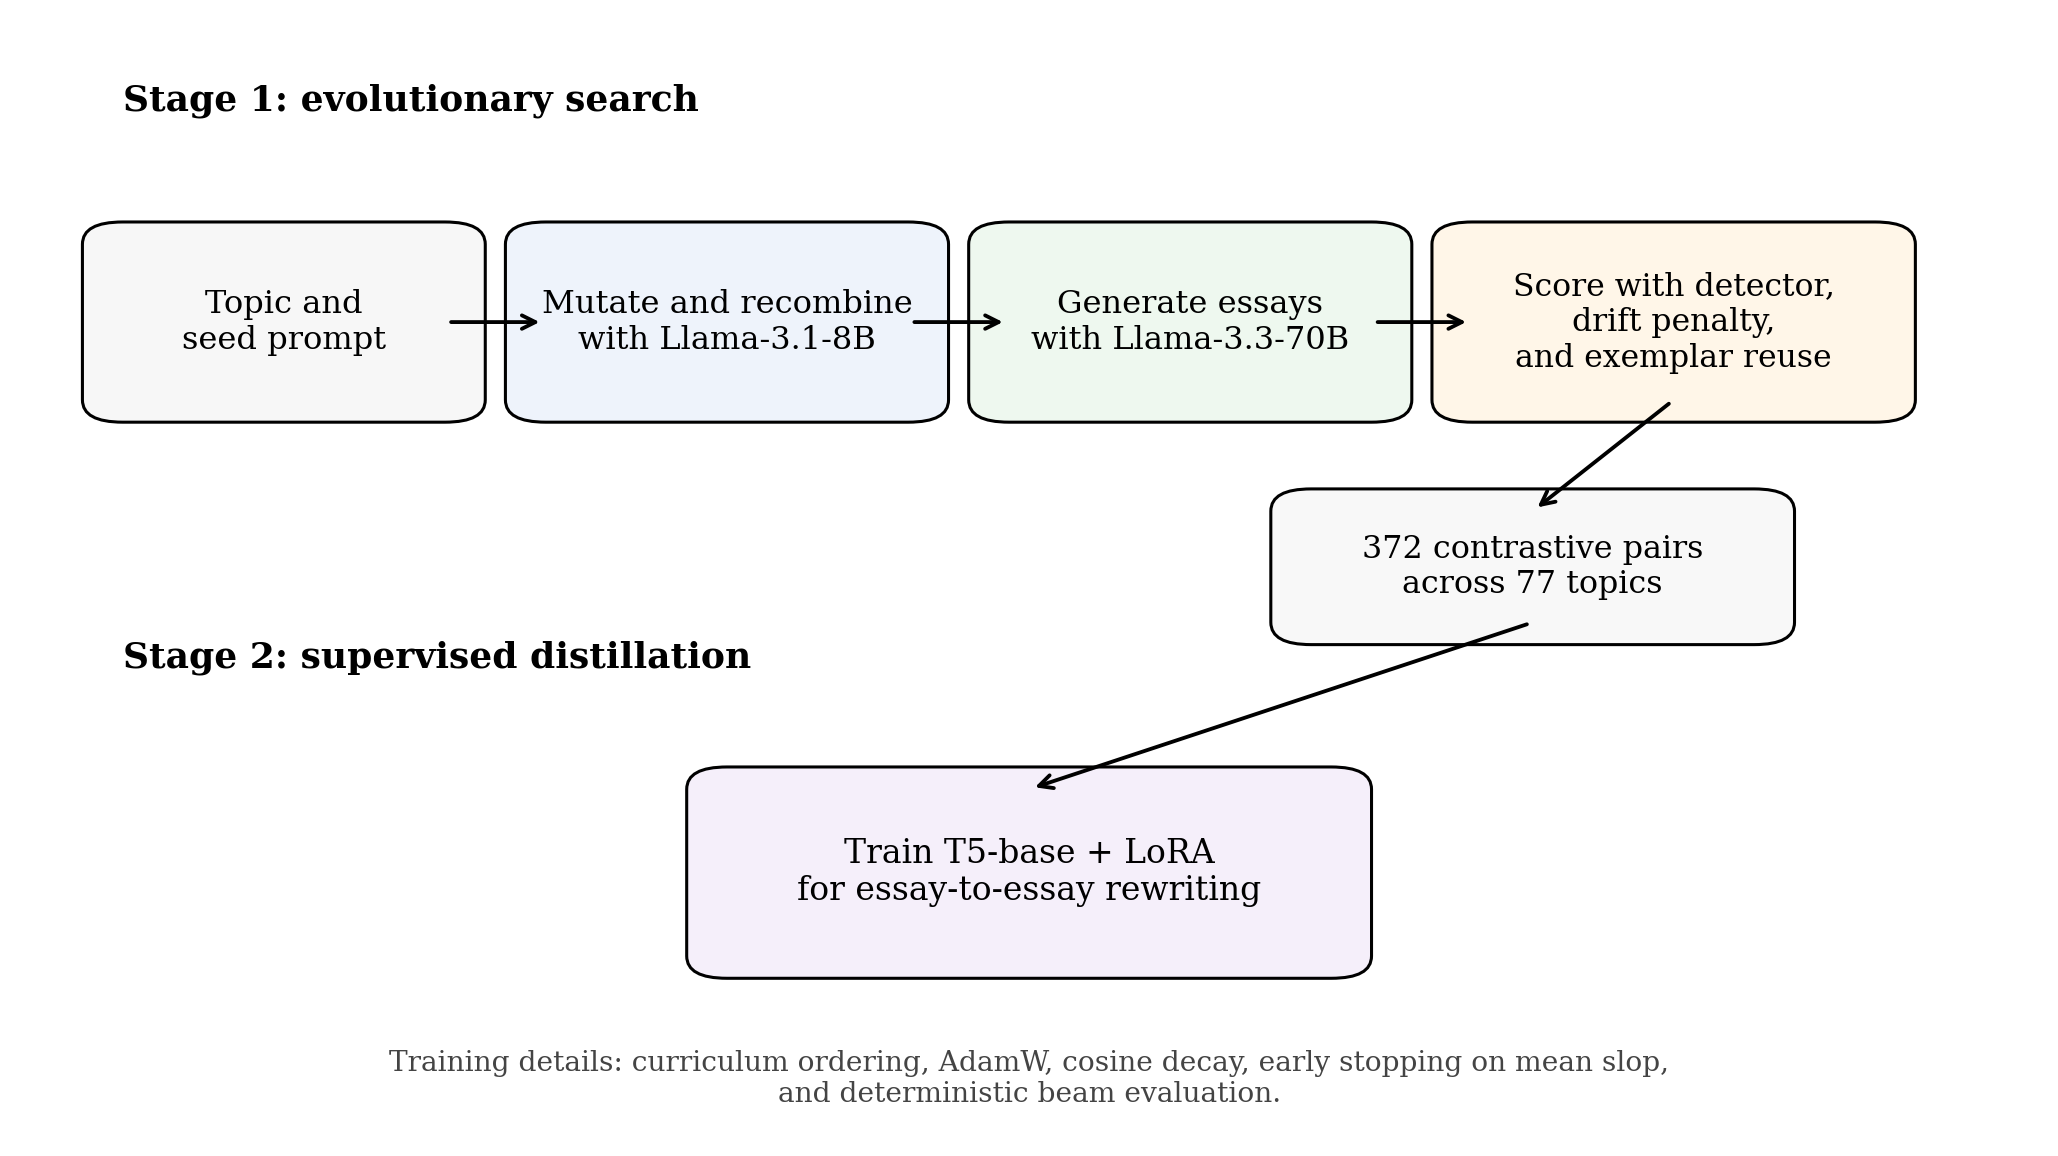
\includegraphics[width=\linewidth]{figures/promptlab_v2_pipeline.png}
\caption{Reconstructed Promptlab-v2 pipeline based on repository code paths and presentation notes. The detector is used first as a search signal and then indirectly through supervised distillation.}
\end{figure}

\subsection{Stage 2: essay-to-essay supervised distillation}

Stage 2 turns those search results into a direct rewriter. The model is T5-base with a LoRA adapter, with the speaker notes reporting roughly 800{,}000 trainable parameters on top of a 220M-parameter backbone. The key architectural change is a shift from prompt-to-prompt optimization to essay-to-essay rewriting. Instead of learning which prompts might later generate low-slop essays, the model learns to map a high-slop essay directly to a lower-slop essay.

Several training decisions appear to matter:

\begin{itemize}[leftmargin=1.2em]
\item AdamW with decoupled weight decay (\texttt{0.01});
\item cosine learning-rate decay from \texttt{1e-4} with 50 warmup steps;
\item curriculum ordering by slop gap, so the model sees the most contrastive pairs first;
\item early stopping on the task metric (\texttt{slop\_mean}) rather than pure cross-entropy;
\item deterministic beam search during evaluation for stable checkpoint comparison.
\end{itemize}

This branch is conceptually important because it offers an offline alternative to direct online reward optimization. The expensive search happens once, and the resulting rewrite model can then run in a single forward pass.

\subsection{Results and limitations}

The final Promptlab-v2 model is the strongest detector-specific performer reported in the repository. On 20 held-out validation pairs, the best configuration achieves mean slop \texttt{0.0998}, compared with a \texttt{0.391} prompt-rewriting baseline, for a 74\% reduction. The best run uses \texttt{LR = 1e-4}, \texttt{r = 16}, and \texttt{weight\_decay = 0.01}; an \texttt{r = 8} ablation reportedly finishes only \texttt{0.006} behind.

These gains come with two critical caveats. First, the dataset is extremely small. The stage-2 best run is ultimately trained on only 40 training pairs with 20 validation pairs, which the presentation explicitly identifies as the binding constraint. The reported ``step-50 noise floor'' is consistent with a high-variance small-data regime. Second, the model is visibly biased toward summarization. The example-essay analysis in the presentation notes indicates that the T5 system often achieves low detector scores by compressing the essay into a shorter text, not by preserving full essay length and rhetorical breadth. That is not a trivial flaw: if the user task is full-length rewriting, then compression is a form of partial task failure even when detector evasion improves.

\begin{figure}[t]
\centering
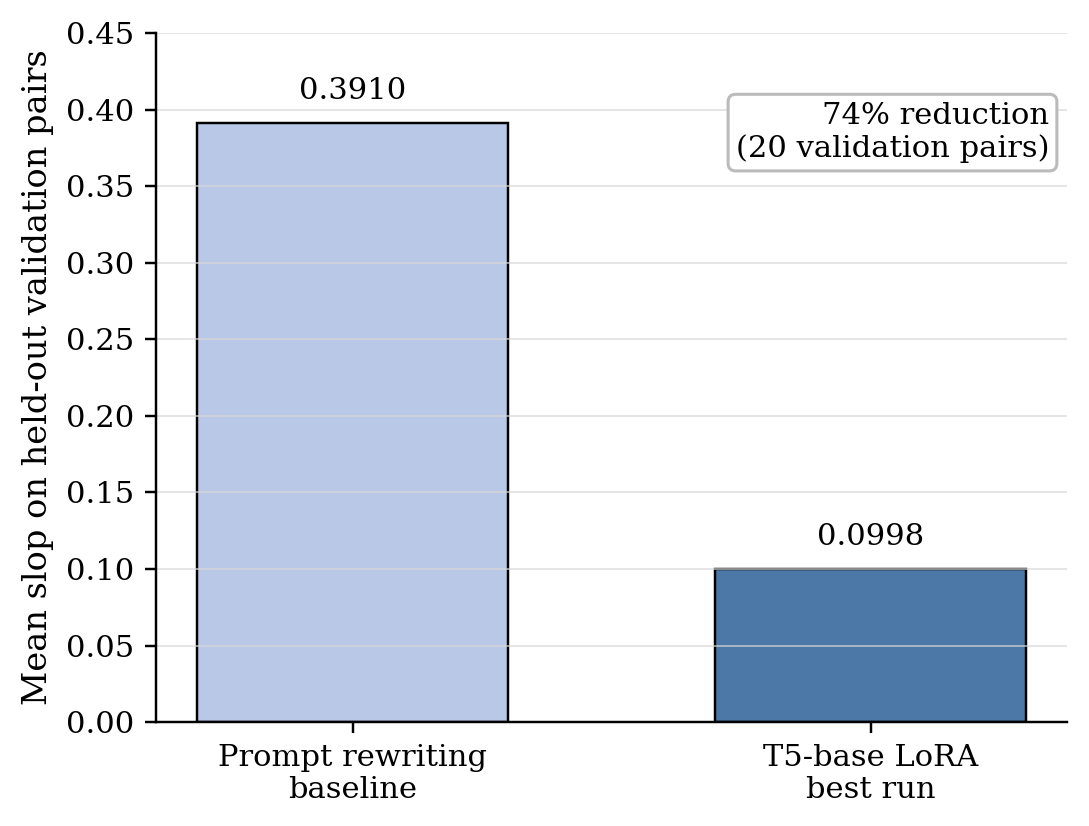
\includegraphics[width=0.72\linewidth]{figures/promptlab_v2_results.png}
\caption{Promptlab-v2 validation result summarized from the project notes: a 74\% reduction in mean slop relative to the prompt-rewriting baseline on 20 held-out validation pairs.}
\end{figure}

This branch therefore provides a compelling proof of concept for offline data-generation and distillation, but not yet a detector-agnostic final answer.

\section{Comparative Discussion}

\subsection{What the three workstreams jointly show}

The repository's main scientific lesson is that deslopification is real but brittle. Each workstream contributes a different piece:

\begin{itemize}[leftmargin=1.2em]
\item The tournament shows that common constraints are necessary, because otherwise detector-aware systems can win for the wrong reasons.
\item The RL branch shows that direct online reward optimization can move a strong detector by a large amount, but it is vulnerable to reward hacking.
\item The Promptlab-v2 branch shows that expensive search can be distilled into a lightweight supervised model, but only under a detector-specific regime and with substantial output-length bias.
\end{itemize}

Across all three, the theme is the same: raw optimization power is not enough. Objective design, regularization, and evaluation discipline determine whether a lower detector score corresponds to a better rewrite.

\subsection{Why the workstreams are not numerically interchangeable}

It would be tempting to read the Promptlab-v2 result (\texttt{0.0998}) as dominating the RL result (\texttt{0.670}). That conclusion would be incorrect. The branches differ in detector family, data regime, and validation structure. Promptlab-v2 is best interpreted as showing that offline search plus distillation can be highly effective on its chosen detector and curated pair set. The RL branch, by contrast, is the strongest evidence that large-scale end-to-end detector reward can move a modern external judge on held-out essays. The tournament sits between them as an attempt to standardize that comparison, and its negative results should be understood as a warning that cross-method evaluation is harder than it looks.

\subsection{Ethics and responsible framing}

This repository studies detector evasion, which has obvious misuse potential. The strongest academically defensible framing is not ``how to bypass detectors in production,'' but rather ``how optimization behaves against imperfect reward models and what failure modes that exposes.'' On that framing, the project is valuable precisely because it shows how easy it is to overfit a detector and how necessary human and multi-detector evaluation are before making claims about genuine writing quality.

\section{Conclusion}

The PromptLab repository contains a coherent body of work on optimization against AI detectability, but it does not support a simplistic victory narrative. The Pangram tournament contributes a rigorous shared harness and exposes how many apparent improvements disappear under fidelity constraints. The REINFORCE deslopifier provides the clearest external-detector result, moving mean EditLens from 0.999 to 0.670 and shifting nearly half the evaluation set out of the fully-AI region, while simultaneously documenting concrete reward-hacking cases. The Promptlab-v2 branch demonstrates that detector-guided search can be distilled into a lightweight essay-to-essay model with very strong detector-specific gains, though on a different judge and with clear summarization bias.

The most defensible synthesis is therefore this: AI-detection evasion is an optimization problem with real signal, but the scientific bottleneck is objective validity, not optimization capability alone. Future progress should unify these workstreams under common judges, larger contrastive datasets, stronger semantic constraints, and human evaluation.

\begin{thebibliography}{9}

\bibitem{thai2025editlens}
K. Thai, B. Emi, E. Masrour, and M. Iyyer.
\newblock EditLens: Quantifying the Extent of AI Editing in Text.
\newblock ICLR 2026 / arXiv:2510.03154.

\bibitem{williams1992reinforce}
R. J. Williams.
\newblock Simple statistical gradient-following algorithms for connectionist reinforcement learning.
\newblock \emph{Machine Learning}, 1992.

\bibitem{hu2021lora}
E. Hu, Y. Shen, P. Wallis, et al.
\newblock LoRA: Low-Rank Adaptation of Large Language Models.
\newblock 2021.

\bibitem{raffel2020t5}
C. Raffel, N. Shazeer, A. Roberts, et al.
\newblock Exploring the Limits of Transfer Learning with a Unified Text-to-Text Transformer.
\newblock \emph{JMLR}, 2020.

\bibitem{rafailov2023dpo}
R. Rafailov, A. Sharma, E. Mitchell, et al.
\newblock Direct Preference Optimization: Your Language Model is Secretly a Reward Model.
\newblock 2023.

\end{thebibliography}

\end{document}
